\documentclass{article}

% - Specify Packages
\usepackage{showkeys}
\usepackage{amssymb}
\usepackage{amsmath}
\usepackage{hyperref}
\usepackage{color}
\usepackage{graphicx}


% ------
\title{TMATH 498: W Doodle}
\author{Rain Wilson}
\date{12 July 2020}

% ------
\begin{document}
\maketitle

% ------
\section{A Piece of the Big Dub}
Figure \ref{fig:my_label} is a rough image placeholder that shouldn't be sharing the same name as Figure \ref{figRect4by8}.
\newline %hi!!!
\begin{figure}[h]
    \centering
    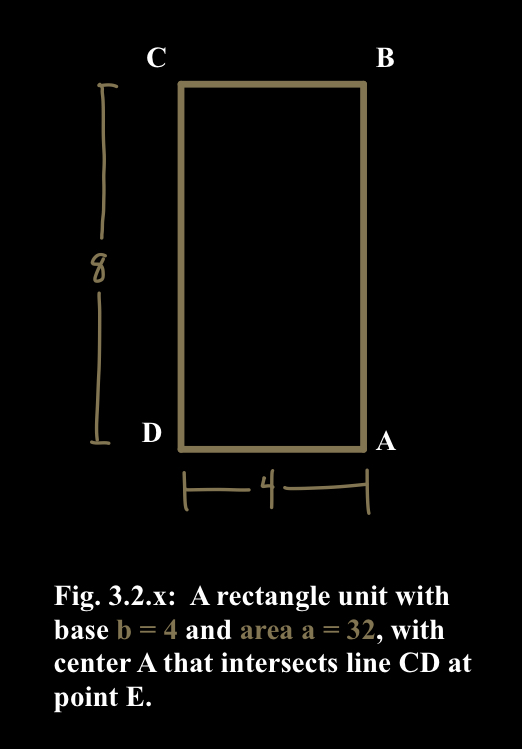
\includegraphics[width=5cm]{  Capstone Presentation/IMG_0004.jpeg}
    \caption{A rectangle unit with....} 
    \label{figRect4by8}
\end{figure}

Why would I possibly want to label things internally when I can just refer to the figure above... well, how about Figure \ref{figRect4by8}
\newline
\begin{figure}
    \centering
    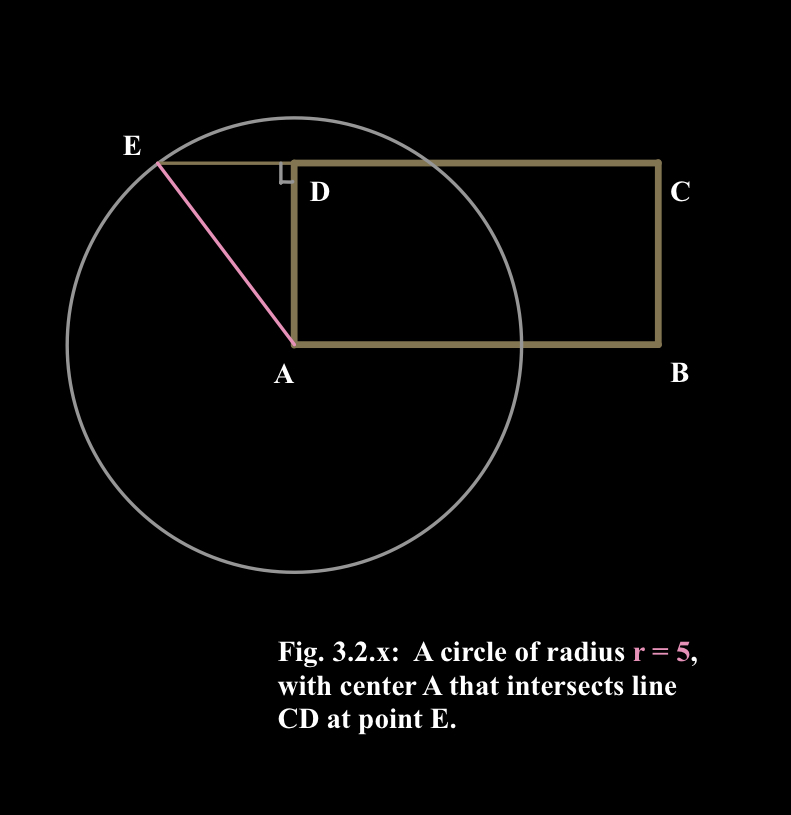
\includegraphics[width=7cm]{Capstone Presentation/IMG_0005.jpeg}
    \caption{Caption}
    \label{fig:my_label}
\end{figure}
\\

% ------

If you want to include pictures of your cat as is shown in Figure \ref{fig:chaos}, you can do that, too.
\begin{figure}
    \centering
    \includegraphics[width=5cm]{Capstone Presentation/chaos.jpeg}
    \caption{If you don't get that phone out of my face, you're going to eat it.}
    \label{fig:chaos}
\end{figure}
\\

She loves to hide under blankets as you can see in Figure \ref{fig:youcantseeme}. It was a hot summer day when I walked around to my side of the bed and saw her like this.
\begin{figure}
    \centering
    
\includegraphics[width=5cm]{Capstone Presentation/youcantseeme.jpeg}
    \caption{These aren't the cats you're looking for.}
    \label{fig:youcantseeme}
\end{figure}

\end{document}